\documentclass[10pt,twocolumn]{article}
\usepackage[margin=0.6in]{geometry}
\usepackage{graphicx}
\usepackage{booktabs}
\usepackage{amsmath}
\usepackage[dvipsnames]{xcolor}
\usepackage{titlesec}
\usepackage[font=footnotesize,labelfont=bf]{caption}
\usepackage{lmodern}
\usepackage{microtype}
\usepackage{stfloats}

\definecolor{ink}{HTML}{0A1638}
\definecolor{navy}{HTML}{2E5CA6}
\definecolor{amber}{HTML}{D97706}
\titleformat*{\section}{\large\bfseries\color{ink}}
\titleformat*{\subsection}{\normalsize\bfseries\color{ink}}
\setlength{\parskip}{2pt}
\renewcommand{\topfraction}{0.95}
\renewcommand{\dbltopfraction}{0.95}
\renewcommand{\textfraction}{0.05}
\renewcommand{\dblfloatpagefraction}{0.90}
\setcounter{dbltopnumber}{3}

\title{\vspace{-1.2em}\textbf{Embedding Agentic Traces}\\[2pt]
\large A trace representation should be faithful to content and invariant to authorship}
\author{Helivan Research --- working summary, August 2026}
\date{}

\begin{document}
\maketitle

\section*{The problem}
Modern evaluation produces \emph{trajectories}: an agent works on a software
issue for tens of minutes and leaves a log of $10^4$--$10^5$ tokens. Public
archives already hold them at scale (SWE-bench Verified: $\sim$119 systems
$\times$ 500 instances, in dozens of incompatible formats), yet each run is
reduced to one pass/fail bit. The obvious move---feed traces to an
off-the-shelf embedder---measures the wrong thing: raw trace embeddings are
\emph{fingerprint readers}. Nearest neighbors are same-system 68--83\%,
same-scaffold at $5\times$ chance, and the exact agent configuration is
retrievable at $0.82$ vs.\ $0.43$ chance even among same-model, same-harness
siblings---while outcome coherence sits at chance (AUC $0.52$). Geometric
fixes fail: per-instance centering alone \emph{amplifies} provenance
dominance ($0.68\!\to\!0.83$), and a dozen unsupervised variants of the naive
representation are performance-identical---an information ceiling.

\section*{qubric: similarity as an input}
For each instance, an LLM reads the \emph{public problem statement} (no
labels) and writes a query-specific rubric: what understanding, localization,
reproduction, editing, verification, and final state concretely mean for
\emph{this} issue. A judge LLM reads each trace through the rubric and
extracts a short factual description per section; sections are embedded
separately, centered against the cross-system median per instance
(consensus centering), and concatenated. The
rubric is a natural-language definition of the equivalence relation the space
should respect; invariance comes from \emph{re-observation through a
fingerprint-poor channel}, not surgery on a fingerprint-rich one.

\begin{figure*}[t]
  \vspace{-6pt}\centering
  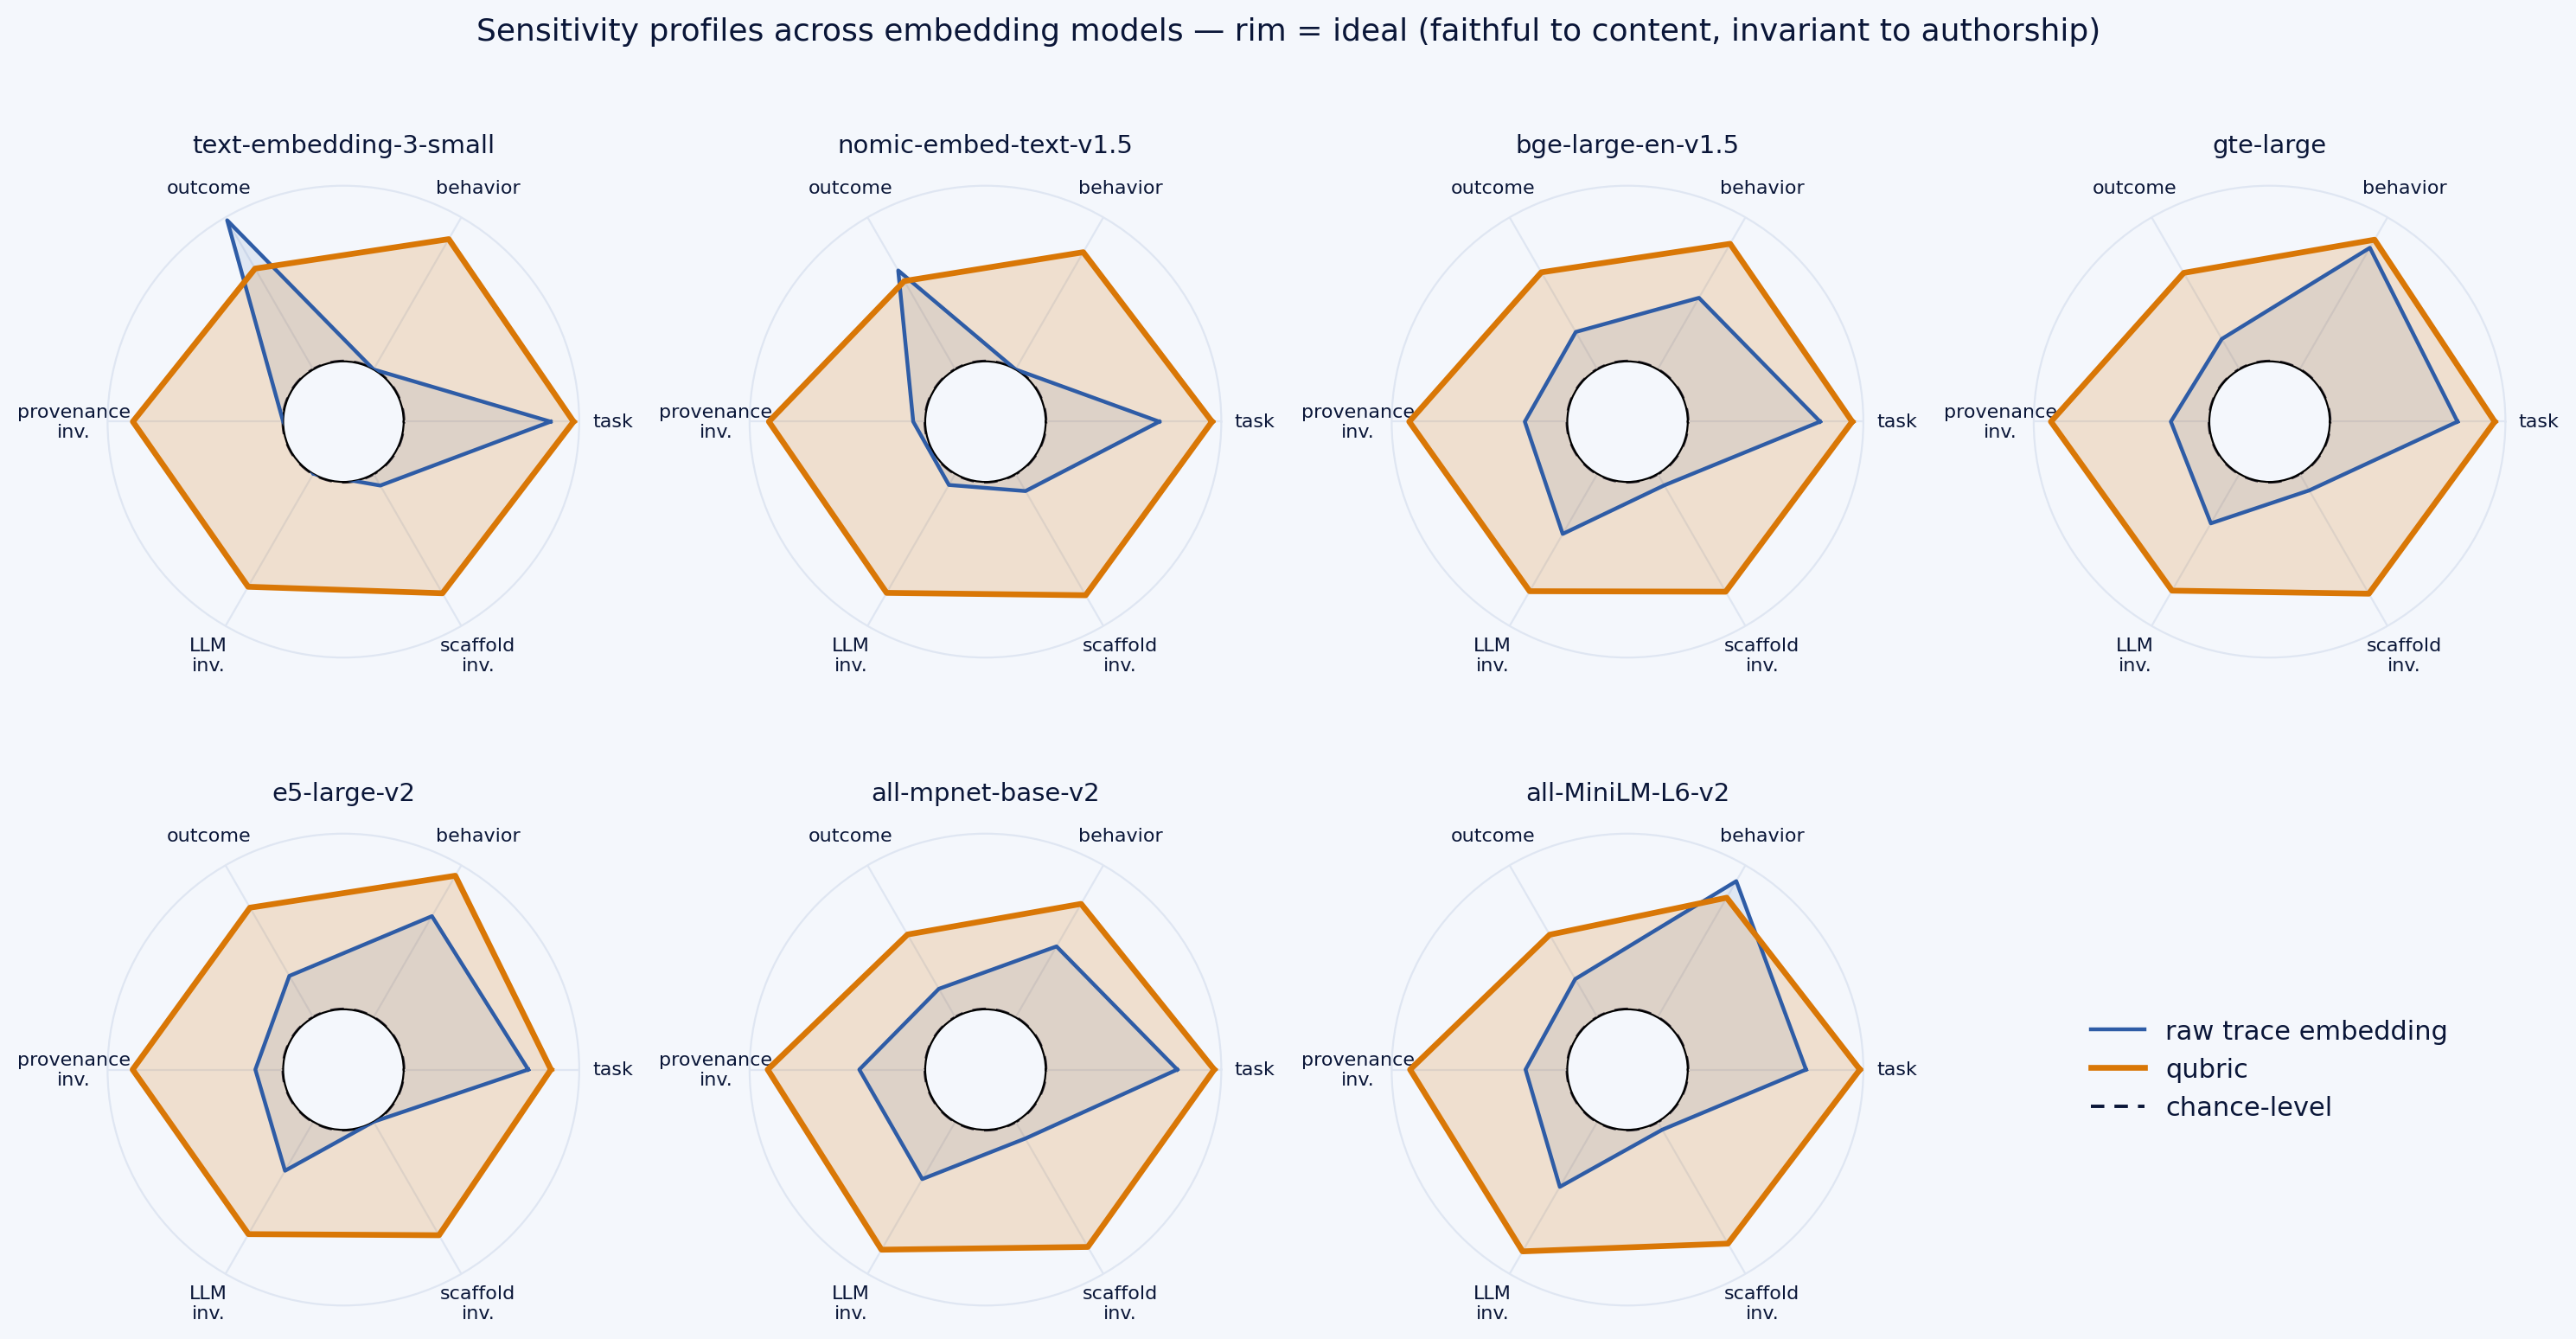
\includegraphics[width=0.72\textwidth]{../figures/radar_all.png}
  \caption{Sensitivity radars across seven embedders. Outside = desirable.
  Raw embeddings (navy) are authorship-dominated; qubric (amber) collapses
  Identity / Model family / Harness to chance while holding Task and
  Behavior.}
  \label{fig:radar}
\end{figure*}
\section*{Evidence: the right sensitivity profile}
Across \textbf{seven embedders} (three families, two orders of magnitude of
size) qubric produces the same profile shift: task fidelity retained
($\sim$0.95), behavior retained or improved, and every authorship axis
collapses to $\approx$chance: provenance $0.83\!\to\!0.09$, scaffold
$0.31\!\to\!0.08$, model lineage $0.20\!\to\!0.12$
(Fig.~\ref{fig:radar}). Pillar independence is verified by double
dissociation across six representations. The instance-conditioning is the
active ingredient---the construction ranking is strict under both readouts
(qubric $>$ verdict questions $>$ generic rubric $>$ free-form summary $>$
raw) and reproduces under a local embedder. No single rubric section carries
the effect (best single section 0.091 vs.\ 0.078 for the union).

\textbf{Judge robustness}: quality degrades
gracefully with judge capability; an open frontier judge
(DeepSeek-v3.1: $0.083/0.079$) matches the closed reference
(gpt-5.4-mini: $0.078/0.078$) within panel resolution, and construction
beats capability---a weak judge \emph{with} a qubric outperforms a strong
judge without one. \textbf{Reliability is measured}: two judges agree on a
single trace only 12--28\% of the time, but aggregating $\sim$20 instances
drives system-level agreement to 0.82--0.95. Per-trace noisy, per-agent
reliable---and per-agent is what evaluation uses.

\begin{figure*}[b]
  \centering
  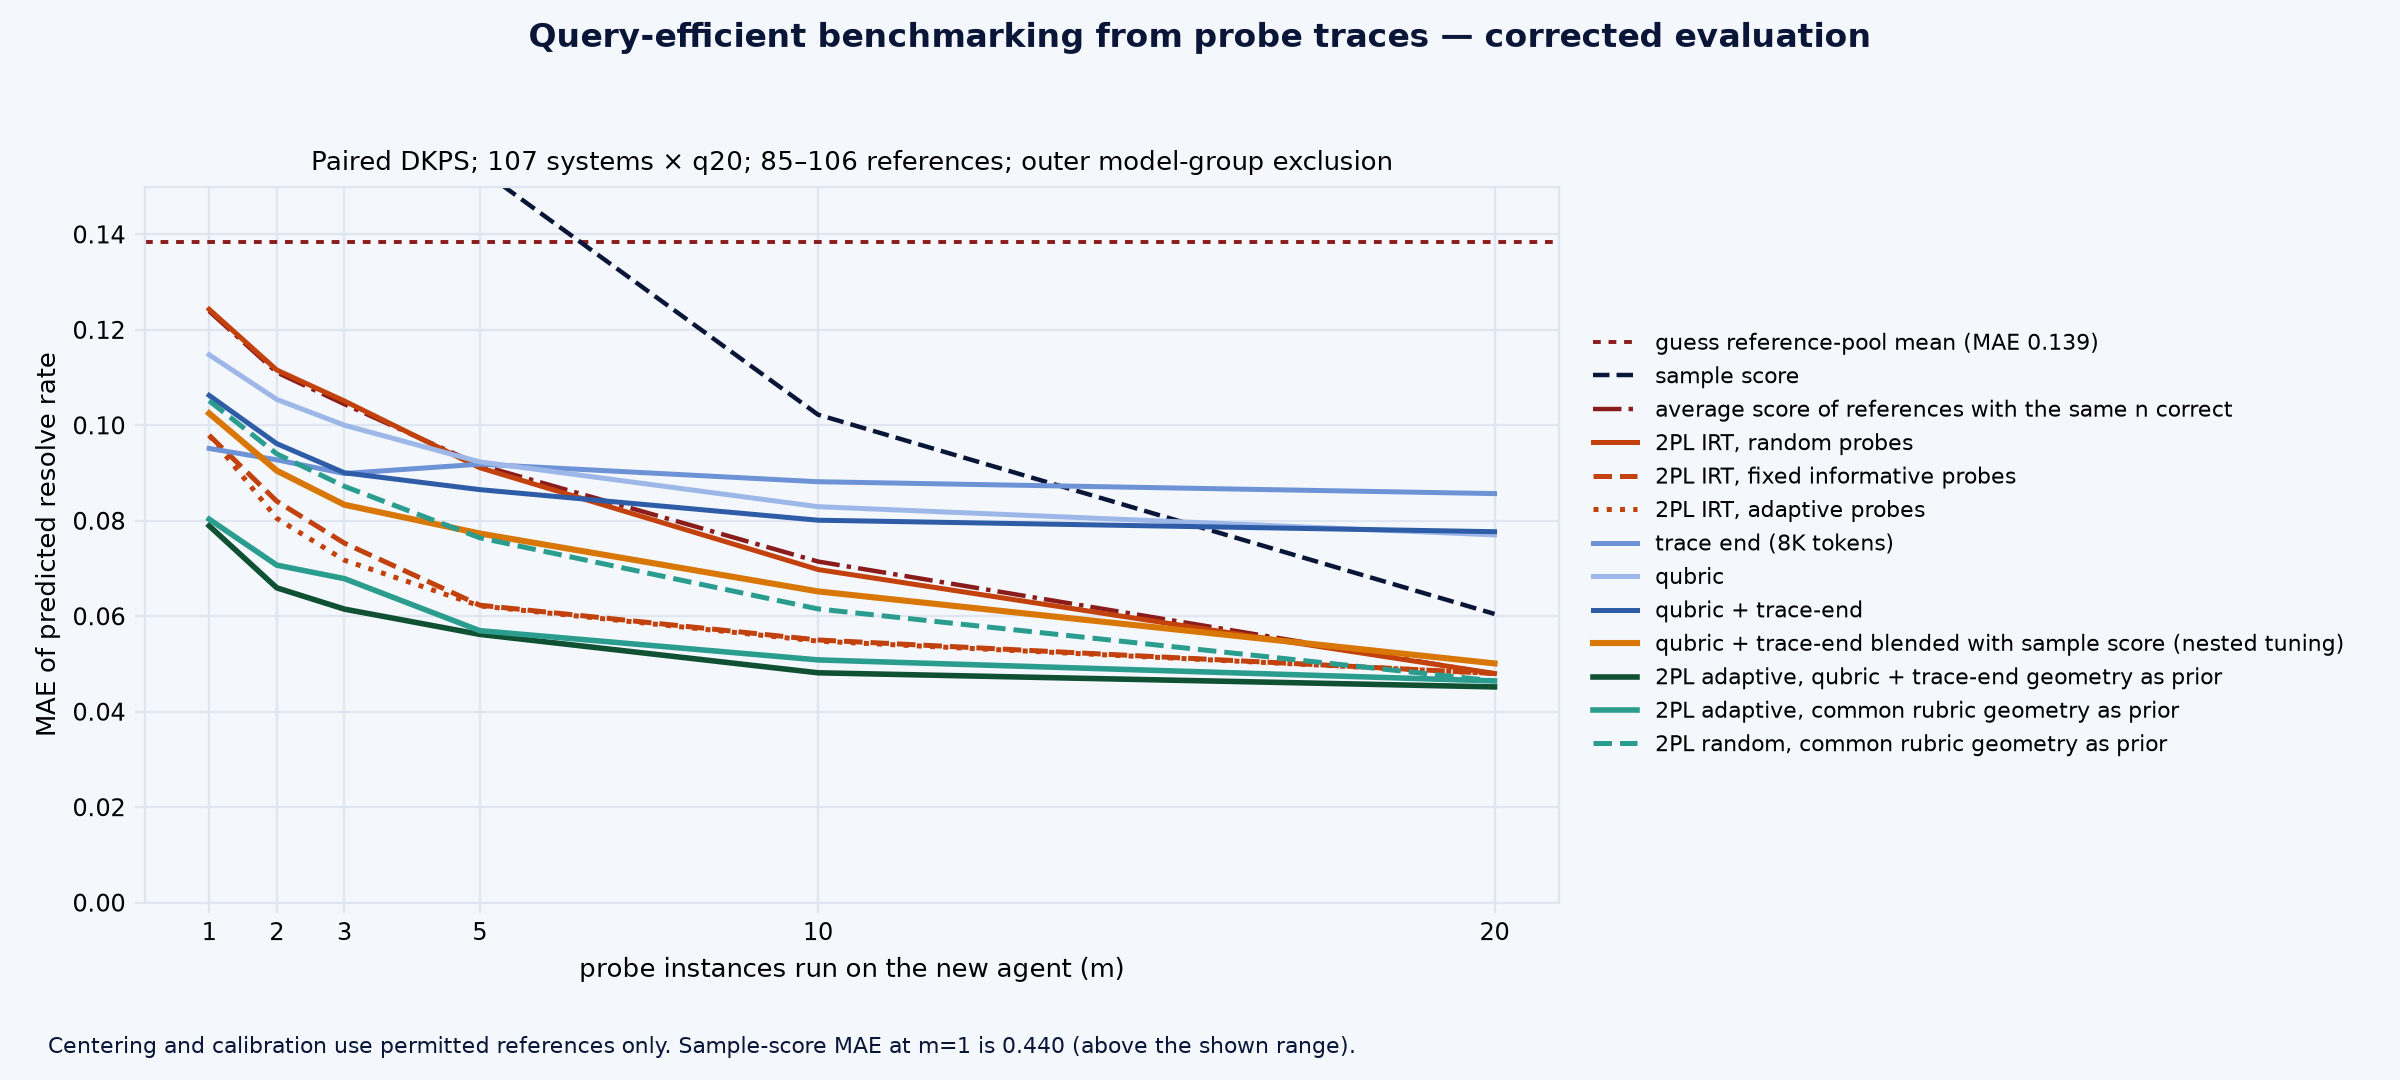
\includegraphics[width=0.86\textwidth]{../figures/fig4_quench.png}
  \caption{QUENCH: error predicting true resolve rates vs.\ probe budget $m$
  (left) and vs.\ reference-pool size $n$ (right); leave-one-LLM-out, 107
  systems.}
  \label{fig:quench}
\end{figure*}
\section*{Payoff: query-efficient benchmarking}
Qubric representations enter the DKPS/PKPS perspective space; a new agent's
full-benchmark resolve rate is predicted from a few probe traces against
references' cached coverage, blended with the sample score. Evaluation is
leave-one-LLM-out throughout (naive CV inflates accuracy $\sim$25\% via
model-family leakage).

\begin{table}[h]
\centering\small
\begin{tabular}{lccc}
\toprule
probes $m$ & sample score & qubric pipeline & +selection \\
\midrule
1  & 0.44 & \textbf{0.095} & --- \\
5  & 0.16 & \textbf{0.074} & 0.057 \\
20 & 0.06 & \textbf{0.048--0.053} & 0.053 \\
\bottomrule
\end{tabular}
\caption{MAE predicting true resolve rates (107 systems). One probe trace
$\approx$ 8--10 scored runs.}
\end{table}

One trace carries far more than one bit: the strongest correctness-only
competitor (CAPA-style error overlap) needs 15--20 \emph{scored} probes to
match one \emph{trace} (0.37 MAE at $m{=}1$), and trails the ensemble at
every budget. The reference pool, not probe count, is the binding resource:
error falls $0.145\!\to\!0.078$ as the pool grows 5$\to$96, still declining
(Fig.~\ref{fig:quench}). Every layer is ablated; CV-inside-selection and
PCA-composed-with-selection are documented overfitting traps.

\subsection*{Status \& caveats}
All qubric numbers: 20-instance panel, one benchmark; differences
${<}0.01$ near panel resolution. The 150-instance scale-up is specified and
unblocked (open-judge stack validated via OpenRouter; $\sim$\$40--85).
Terminal-Bench (142 systems, 89 tasks, $\geq$5 trials/task, public
trajectories) is scoped and deferred. Full log: \texttt{FINDINGS.md}
(F1--F24) on the \texttt{agentic-traces} branch.




\end{document}
